% LTeX: language=de-DE
\section{Konzepte}
Die theoretischen Grundlagen des Konzepts der Schwarmintelligenz in der Robotik werden in diesem Kapitel erläutert und in Bezug auf eine Anwendung mit Raspberry Pi Einplatinencomputer gebracht. Diese sollen durch einen zufällig generierten Hindernis-Parcours fahren und die vorhandenen Hindernisse hierbei umfahren. Zudem soll durch mehrere Iterationen an Durchläufen die Effizienz der Lösung verbessert werden. Für die Umsetzung und die Lösung des Problems wurden mehrere Ideen und Ansätze entwickelt und in diesem Kapitel erläutert und miteinander verglichen. Außerdem werden die einzelnen Komponenten des Konzepts erläutert und die einzelnen Schritte der Implementierung beschrieben. Die Problemstellung bei allen Konzepten soll sein, dass eine durch X- und Y-Koordinaten definierte Strecke mit einem Hindernis-Parcours so verarbeitet wird, dass durch diese ein Pfad gefunden wird, der Hindernisse vermeidet. Außerdem soll aus diesen gefundenen Pfaden der effizienteste Pfad ermittelt werden.

\subsection{Umsetzung des Konzepts ausschließlich in Code}
Die Umsetzung des Konzepts in Code ist die einfachste und schnellste Möglichkeit, um das Konzept in die Realität umzusetzen. Allerdings ist diese Variante verglichen mit einer Umsetzung mit Hardware weniger realitätsnah und weist einen geringeren Bezug zum eigentlichen Problem, der mobilen Schwarmintelligenz, auf. Für diesen Ansatz werden keine Hardware-Komponenten benötigt. Das zu lösende Problem soll mithilfe eines künstlichen Schwarmes einen Pfad zu finden, der Hindernisse vermeidet umgesetzt werden. Als Programmiersprache soll Python verwendet werden, da Python durch diverse Module und Bibliotheken, wie zum Beispiel Numpy, Matplotlib oder Scipy, einen Vorteil gegenüber anderen Programmiersprachen bietet, mit denen sich die Umsetzung des Konzepts umständlicher umsetzen ließe. In Code Darstellung \autoref{lst:marix-gen} wird eine Methode für die Erstellung einer 20x20 Matrix exemplarisch dargestellt. Eine solche Matrix kann als eine Art "Karte" verstanden werden, auf der Hindernisse und Wege dargestellt werden können. Die Matrix wird mit Nullen initialisiert und an den Stellen, an denen Hindernisse sein sollen, mit Einsen belegt. Mit den exemplarischen Parametern werden 18 Hindernisse zufällig gesetzt. Die Matrix wird anschließend ausgegeben.

%minted python code
\begin{minted}{python}
import numpy as np

def obstacles():
    """
    Creates a 20x20 grid with obstacles randomly placed.
    Grid containing 1 is an obstacle, containing 0 is empty.
    Returns a numpy array of the grid.
    """
    obs = np.zeros((20,20))
    for i in range(18):
        obs[np.random.randint(20)][np.random.randint(20)] = 1  
  
    return obs
\end{minted}
\vspace*{-3mm}
\captionof{listing}{\label{lst:marix-gen}Matrizen Generierung}
\vspace*{3mm}

Die Abbildung, die mit dem Python Package \textit{matplotlib} erstellt wurde, visualisiert eine Matrix, die durch die in Code Darstellung \autoref{lst:marix-gen} dargestellte Funktion erstellt wurde. Der Startpunkt ist bei den Koordinaten (0/0) als grüner Punkt angezeigt. Das Ziel am Punkt (20/20) als roter Punkt. Die weiße Fläche stellt den freien und somit durchquerbaren Bereich und die schwarzen Flächen den durch Hindernisse blockierten dar. Diese Daten sind die Ausgangslage für einen darauf angewandten Schwarmintelligenz Algorithmus dar, dessen Output den bestmöglichen Pfad durch diese Fläche ermitteln soll, siehe \autoref{fig:Figure_1}.
\begin{figure}[H]
    \centering
    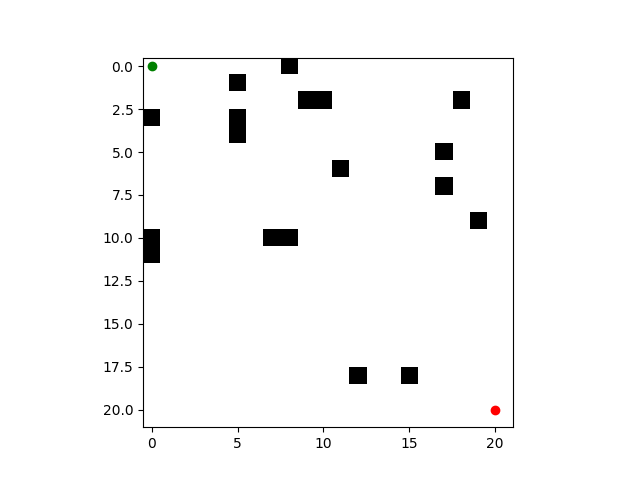
\includegraphics[width=\textwidth]{Figure_1.png}
    \caption{Visualisierung der Matrix}
    \label{fig:Figure_1}
\end{figure}

In Folge der Ermittlung kann der optimale Pfad verwendet werden, um den effizientesten Weg durch die Matrix, beziehungsweise die Hindernisse grafisch darzustellen.

\subsection{Umsetzung des Konzepts in der physischen Variante}
In dieser Implementierung wird ein Schwarmintelligenz-Algorithmus verwendet, um einen optimalen Pfad basierend auf Daten aus der realen Umgebung zu finden. Im Gegensatz zur reinen Code-basierten Variante werden die Daten nicht zufällig generiert, sondern von Sensoren des Roboters in der physischen Umgebung erfasst. Denkbar wären hier beispielsweise die Nutzung von Ultraschallsensoren, die an Einplatinencomputer wie dem Raspberry Pi an den vorhandenen GPIO-Pins angeschlossen werden können. Die Sensoren sammeln regelmäßig Daten, die in einer Datenbank gespeichert und periodisch abgefragt werden könnten, um sie dem Schwarmintelligenz-Algorithmus zur Berechnung des optimalen Pfades zur Verfügung zu stellen. Der Algorithmus liefert dann den optimalen Pfad, den der Roboter durch die Umgebung nutzen kann. Dieser soll dann in der Lage sein, den Pfad so zu durchfahren, dass er nicht mehr auf die Sensoren zur Erkennung der Hindernisse angewiesen ist. Sowohl beim Erlangen der Daten, wobei der Roboter an einem Startpunkt beginnt, die Umgebung zu durchfahren, als auch beim Durchfahren ohne die Sensoren, müssen die Koordinaten des Roboters zum jeweils aktuellen Zeitpunkt bestimmt werden können. Dies ist nur dann möglich, wenn anhand der Umdrehungen der Servomotoren, die zur Fortbewegung genutzt werden, ermittelt werden kann, wie weit und in welche Richtung sich ein Roboter jeweils fortbewegt hat. Für die Ermittlung wird hierfür weiterhin die Größe der verwendeten Räder benötigt. Sind diese beiden Messgrößen bekannt, können anhand dieser die Position und auch Anweisungen zum Fahren übermittelt werden.
\begin{figure}
    \centering
    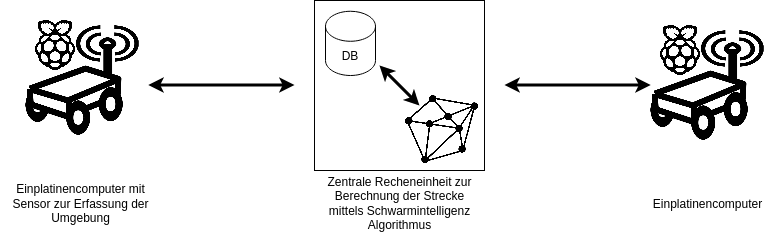
\includegraphics[width=\textwidth]{draw_io_overview_robot.png}
    \caption{Übersicht physische Variante}
    \label{fig:Figure_2}
\end{figure}

Die Qualität der Daten hängt hierbei stark von der verwendeten Hardware ab. Zum einen, weil anhand von Umdrehungen der Servomotoren bestimmt wird, wo sich ein Roboter zum jeweiligen Zeitpunkt befindet und zum anderen von der Genauigkeit der verwendeten Ultraschallsensoren, wenn diese Hindernisse in ihrer Umgebung detektieren. Als zusätzlicher Schritt, welcher bei der Code-basierten Variante nicht anfällt, ist es in dieser Umsetzung notwendig, die erfassten Daten in eine Form zu bringen, die der Schwarmintelligenz-Algorithmus verarbeiten kann. Denkbar wäre hier ebenfalls die Nutzung von Bibliotheken wie beispielsweise `numpy`, um eine Matrix in der Größe des Kartenbereichs zu erstellen. Anhand der aktuellen Position des erfassenden Raspberry Pi Roboters könnten in Abhängigkeit des Abstands zu einem Hindernis die entsprechenden X- und Y-Koordinaten in der Matrix auf 1 gesetzt werden. Eine solche Matrix könnten dann wie in der Code-basierten Variante an den Schwarmintelligenz-Algorithmus zur Verarbeitung übergeben werden.

\subsection{Umsetzung des Konzepts hybrider Variante}
Bei der Umsetzung in hybrider Variante handelt es sich um ein gemischtes Vorgehen aus der reinen Code-basierten Variante und der physischen Variante. Die Daten der zu verarbeitenden Umgebung werden wie bei der Code-basierten Variante durch einen Algorithmus generiert. Nach Verarbeitung der Daten erfolgt jedoch ein Schritt in die physische Umsetzung. Der durch den verwendeten Schwarmintelligenz Algorithmus ermittelte Pfad wird nach der Verarbeitung in Instruktionen übersetzt, die der Roboter in der physischen Umgebung ausführen kann. Hierfür ist eine Verbindung zwischen dem Algorithmus und dem Roboter notwendig. Diese kann beispielsweise durch eine WLAN-Verbindung hergestellt werden. Weiterhin muss eine Schnittstelle geschaffen werden, über welche der Client, der den Algorithmus und die Berechnungen ausführt, mit dem Roboter kommunizieren kann. Wenn auf das Kriterium der Echtzeit verzichtet werden kann, eignet sich hierfür eine reguläre API Schnittstelle. Der Raspberry würde in diesem Fall einen Endpunkt darstellen, an den Instruktionen in Form des gewählten Datenformats wie beispielsweise JSON oder XML gesendet werden. Diese Schnittstelle würde sich zudem auch für die Übermittlung von Signalen wie Start, Stopp oder Reset eignen.
\begin{figure}[H]
    \centering
    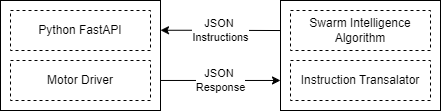
\includegraphics[width=\textwidth]{hybrid-diagram.png}
    \caption{Übersicht hybride Variante}
    \label{fig:overview-hybrid}
\end{figure}

\section{Auswahlkriterien für das verwendete Vorgehen}
Bei der Auswahl von Kriterien für den Vergleich zwischen der reinen Code-basierten Implementierung, der physischen Implementierung und der hybriden Implementierung des Konzepts der mobilen Schwarmintelligenz werden die folgenden Aspekte berücksichtigt:
\begin{itemize}
    \item Realitätsnähe: Realitätsnähe im Kontext der Implementierung eines Schwarmverhaltens bezieht sich auf die Fähigkeit der Implementierung, das tatsächliche Verhalten des Schwarmes in der realen Umgebung genau vorherzusagen. Es geht darum, wie nahe die Simulation der realen Umgebung kommt und wie gut die Implementierung die Gegebenheiten und Bedingungen der realen Welt berücksichtigt.
    \item Komplexität: Komplexität im Kontext der Implementierung sowie einer möglichen physischen Umsetzung bezieht sich auf den Schwierigkeitsgrad der Implementierung des Schwarmintelligenz-Algorithmus sowie der physischen Umsetzung. Hierbei werden die Kriterien Programmieraufwand, zusätzlich benötigte Kenntnisse und die Komplexität der benötigten Hardware berücksichtigt.
    \item Kosten: die Kategorie Kosten bezieht sich in erster Linie auf eine Implementierung der physischen Variante. Hierbei werden die Kosten für die benötigte Hardware berücksichtigt. Es soll erwähnt werden, dass eine Implementierung mit bereits vorhandenen und durch die Lehrstätte zur Verfügung gestellten Ressourcen durchgeführt werden soll.
    \item Skalierbarkeit: Skalierbarkeit bezieht sich auf die Fähigkeit der Implementierung, auf größere oder kleinere Umgebungen angepasst zu werden. Das bedeutet, dass die Implementierung in der Lage sein sollte, auf unterschiedliche Schwarmgrößen, räumliche Gegebenheiten, unterschiedliche Sensordaten oder andere Anforderungen anpassbar zu sein.
    \item Geschwindigkeit: Geschwindigkeit bezieht sich in diesem Zusammenhang auf die Fähigkeit des Algorithmus, Eingabedaten schnell zu verarbeiten und Entscheidungen zu treffen. Eine Implementierung mit hoher Geschwindigkeit kann schnell auf Änderungen in der Umgebung oder auf neue Anforderungen reagieren und somit effektiver arbeiten.
    \item Visualisierung: Visualisierung bezieht sich darauf, wie die Ergebnisse der Implementierung dargestellt und realitätsnah dargestellt werden können. Es soll betrachtet werden, wie gut das Verhalten des Schwarmes in der realen Umgebung simuliert werden kann und wie gut die Ergebnisse der Implementierung dargestellt werden können.
\end{itemize}

\begin{table}[H]
    \renewcommand{\arraystretch}{1.2}
    \caption{Entscheidungsmatrix: verwendetes Konzept}
    \label{tab:decision-matrix}
    \begin{tabularx}{\textwidth}{|X|X|X|X|}
        \hline
        & \textbf{Code-basiert} & \textbf{Physisch} & \textbf{Hybrid} \\
        \hline
        \textbf{Kriterium} & Punkte & Punkte & Punkte \\
        \hline
        Realitätsnähe & 1 & 5 & 3 \\
        \hline
        Komplexität & 4 & 1 & 3 \\
        \hline
        Kosten & 5 & 3 & 4 \\
        \hline
        Skalierbarkeit & 4 & 2 & 3 \\
        \hline
        Geschwindigkeit & 4 & 2 & 3 \\
        \hline
        Visualisierbarkeit & 2 & 5 & 4 \\
        \hline
        \rowcolor{gray!50}
        \textbf{Summe} & 20 & 18 & 20 \\
        \hline
    \end{tabularx}
\end{table}

Die Punkte der einzelnen Kriterien wurden in einer Skala von 1 bis 5 vergeben. Dabei steht 1 für die schlechteste Bewertung und 5 für die beste Bewertung. Die Summe der Punkte der einzelnen Kriterien ergibt die Gesamtpunktzahl für das jeweilige Konzept. Die ermittelten Punkte liegen wie in \autoref{tab:decision-matrix} alle sehr nah beieinander. Während die Umsetzung des Vorhabens in der physischen Variante einen erhöhten Aufwand und gegenüber den anderen Vorgehensweisen mit einer deutlich höheren Komplexität einhergeht, bietet sie gleichzeitig die beste Realitätsnähe. Die Umsetzung in der Code-basierten Variante ist hingegen mit einem geringeren Aufwand verbunden, bietet jedoch die geringste Realitätsnähe. Die Umsetzung in der hybriden Variante bietet eine gute Realitätsnähe und ist mit einem vergleichbaren Aufwand verbunden. Eine Umsetzung in der hybriden Variante wird daher als Basis für die weitere Implementierung des Vorhabens verwendet. 

\section{Hardware}
In diesem Abschnitt werden die verwendeten Hardware-Komponenten für die Umsetzung der hybriden Variante beschrieben. Es ist zu erwähnen, dass bei der gewählten und verwendeten Hardware vorzugsweise auf Materialien zurückgegriffen wurde, die bereits durch die Lehrstätte zur Verfügung gestellt wurden. Möglicherweise gibt es bessere Alternativen, die zum Zeitpunkt der Umsetzung jedoch nicht zur Verfügung standen. Die verwendeten Hauptkomponenten sind ein Raspberry Pi 3, ein Grove Base HAT, ein Servo Motor und ein eigens dafür konstruiertes und anschließend mit einem 3D-Drucker angefertigtes Gehäuse, das alle Komponente vereint. Die Komponenten sind in \autoref{fig:hardware} dargestellt.

\begin{figure}[ht]
    \centering
    \begin{subfigure}[b]{0.45\textwidth}
      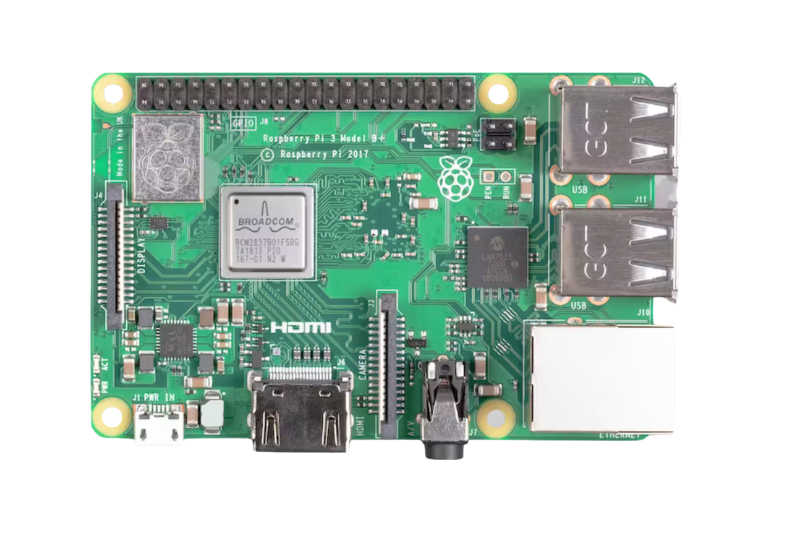
\includegraphics[width=\textwidth]{raspi.png}
      \caption{Raspberry Pi 3 \cite{raspberry-pi}}
    \end{subfigure}
    \hspace{1cm}
    \begin{subfigure}[b]{0.45\textwidth}
      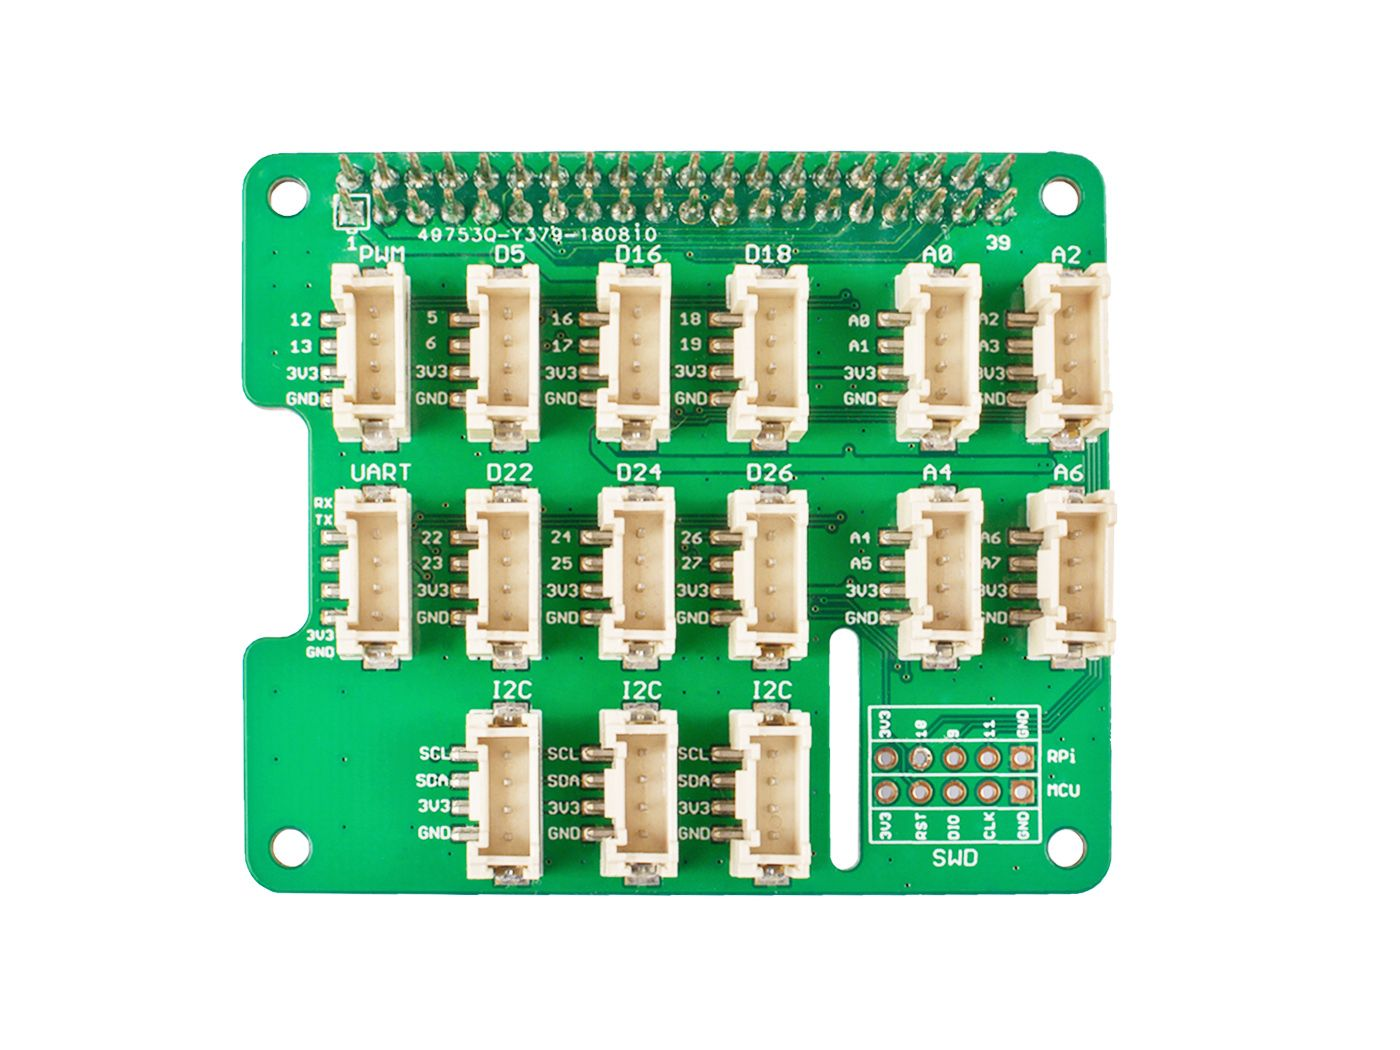
\includegraphics[width=\textwidth]{base-hat.jpg}
      \caption{Grove Base HAT \cite{seeedstudio} \label{fig:base-hat}}
    \end{subfigure}
    \vskip\baselineskip
    \begin{subfigure}[b]{0.45\textwidth}
        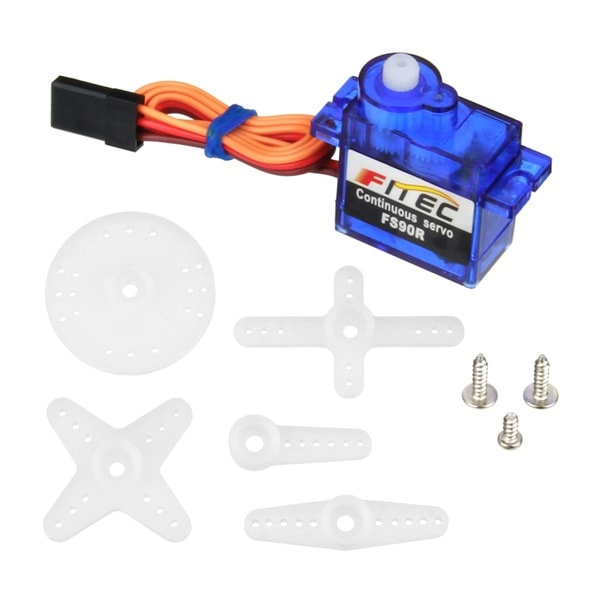
\includegraphics[width=\textwidth]{servo.jpg}
        \caption{Servomotor \cite{addicore_fs90r_micro_servo} \label{fig:servo}}
      \end{subfigure}
      \hspace{1cm}
      \begin{subfigure}[b]{0.45\textwidth}
        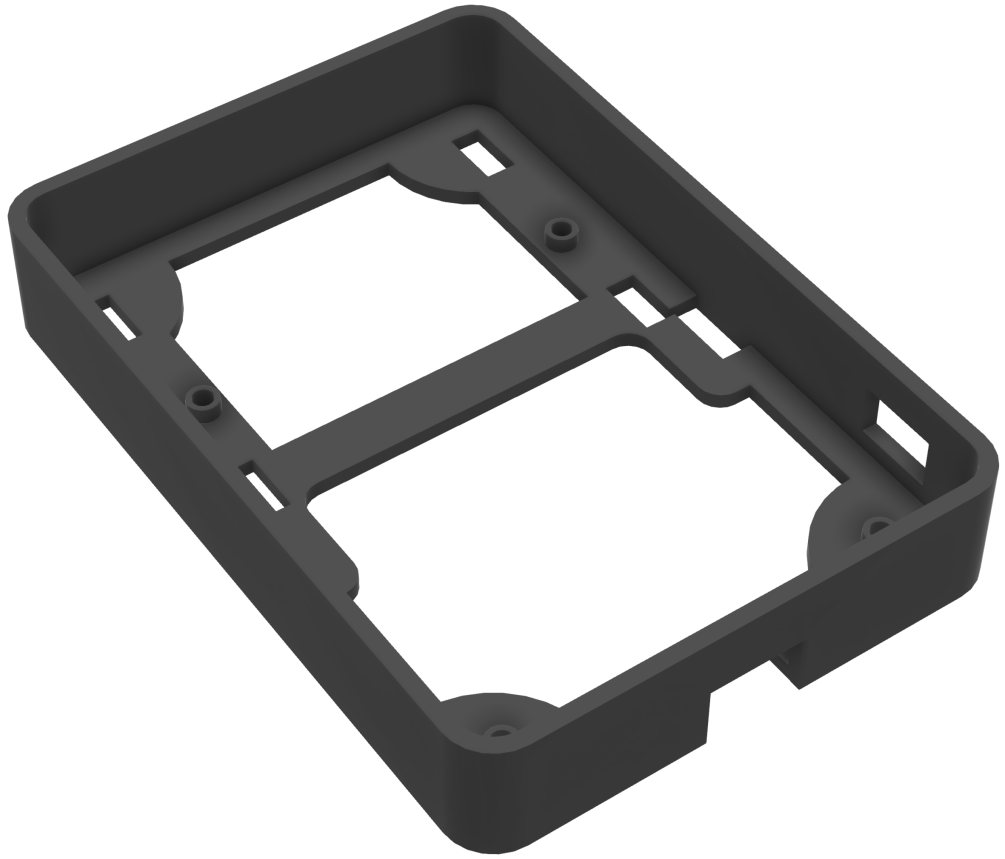
\includegraphics[width=\textwidth]{case.png}
        \caption{Roboter Gehäuse \label{fig:case}}
      \end{subfigure}
    \caption{Verwendete Bauteile \label{fig:hardware}}
\end{figure}

Der Raspberry Pi dient hierbei als Einplatinencomputer, der die Steuerung des Roboters übernimmt. Der Grove Base HAT, in \autoref{fig:base-hat} dargestellt, bietet die Möglichkeit verschiedene Sensoren und Aktoren anzuschließen. Servomotoren, wie in \autoref{fig:servo} dargestellt, dienen hierbei als Antrieb des Roboters. Das Gehäuse, in \autoref{fig:case} dargestellt, vereint alle Komponenten und bietet eine einfache Montage und Demontage der einzelnen Komponenten. Die Wahl des Servomotors ist aufgrund der geringen Größe und der niedrigen benötigten Versorgungsspannung auf ein Modell dieser Bauart gefallen. Außerdem sind diese Art von Servomotoren günstig erhältlich sowie energieeffizient \cite{Sustek2017}. Die Wahl des Grove Base HAT ist aufgrund der einfachen Verwendung und der Möglichkeit, verschiedene Sensoren und Aktoren anzuschließen, auf dieses Modell gefallen. Bei diesem Bauteil handelt es sich um eine Addon Board, das es erlaubt, Bauteile wie Sensoren und Aktoren über einen einfachen Steckverbinder anzuschließen \cite{seeedstudio}.


\section{Steuerung und Kommunikation}
Für die Kommunikation des Roboters stehen verschiedene Übertragungs- und Kommunikationsmöglichkeiten zur Verfügung. Aufgrund der Anforderung, dass das Gerät mobil betrieben werden soll, eignet sich eine kabellose Variante.

Vergleichen werden hierfür die Möglichkeiten MQTT, REST API und Web Socket. Für den Anwendungsfall relevant sind die folgenden Eigenschaften:
\begin{itemize}
  \item Einfache Implementierung
  \item Keine zusätzliche Hardware notwendig
  \item Flexibilität
  \item Skalierbarkeit
  \item Zuverlässigkeit
\end{itemize}

Während sich Kriterien für den Einsatz von Robotik hauptsächlich auf eine hohe Zuverlässigkeit, geringe Latenzen sowie eine hohe Flexibilität beziehen \cite{AMARAN2015400}, werden im Rahmen dieser studentischen Arbeit andere Kriterien als relevant angesehen, mit unter, weil diese für die Umsetzung des Vorhabens eine Erleichterung mit sich bringen. So ist die einfache Implementierung ein wichtiges Kriterium, da die Umsetzung in einer begrenzten Zeit erfolgen soll. Die zu verwendende Hardware soll sich, wenn möglich, auf bereits vorhandene Komponenten beschränken. Flexibilität ist insofern relevant, als bei der Umsetzung des Vorhabens eine hohe Anpassungsfähigkeit an die Umgebung gewünscht ist. Wenn Änderungen notwendig werden, soll diese möglichst einfach umsetzbar sein, ohne dass die gesamte Umsetzung neu durchgeführt werden muss. Skalierbarkeit soll möglich sein, sodass das System bei einer Erweiterung der Anzahl an Geräten, auf das es verteilt wird, in gleicher Weise funktionieren soll. Zuverlässigkeit ist ein wichtiges Kriterium, da die Kommunikation zwischen den einzelnen Geräten nicht unterbrochen werden darf.
\begin{table}[H]
  \renewcommand{\arraystretch}{1.2}
  \caption{Entscheidungsmatrix: Verwendete Kommunikationsprotokolle}
  \label{tab:decision-matrix-communication}
  \begin{tabularx}{\textwidth}{|X|X|X|X|}
      \hline
      & \textbf{MQTT} & \textbf{REST API} & \textbf{Web Socket} \\
      \hline
      \textbf{Kriterium} & Punkte & Punkte & Punkte \\
      \hline
      Einfache Implementierung & 2 & 4 & 3 \\
      \hline
      Keine zusätzliche Hardware & 1 & 5 & 5 \\
      \hline
      Flexibilität & 5 & 3 & 4 \\
      \hline
      Skalierbarkeit & 4 & 4 & 4 \\
      \hline
      Zuverlässigkeit & 5 & 4 & 4 \\
      \hline
      \rowcolor{gray!50}
      \textbf{Summe} & 17 & 20 & 20 \\
      \hline
  \end{tabularx}
\end{table}

Die Punkte der einzelnen Kriterien wurden in einer Skala von 1 bis 5
vergeben. Dabei steht 1 für die schlechteste Bewertung und 5 für die beste Bewertung. Die Summe der Punkte der einzelnen Kriterien ergibt die Gesamtpunktzahl für die jeweilige Technologie.
Obwohl in den Bereichen Robotik und IoT häufig MQTT verwendet wird \cite{AMARAN2015400}, wird es für diese studentische Arbeit nicht in Betracht gezogen. Nicht zuletzt, weil keine Vorkenntnisse der Bearbeitenden vorhanden sind.

\subsection{REST API}
Unter Einbeziehung der in \autoref{tab:decision-matrix-communication} aufgezeigten Ergebnisse der Entscheidungsfindung für eine geeignete Möglichkeit der Kommunikation mit dem verwendeten Raspberry Pi Einplatinencomputer, fällt die Wahl für die Implementierung einer REST API Schnittstelle auf die in Python zu implementierende Lösung \textit{FastAPI} \cite{tiangolo_fastapi_features}. In \autoref{fig:apidocs} werden die für das Vorhaben benötigten API-Endpunkte in Form einer durch die Umsetzung automatisch generierten API-Dokumentation aufgezeigt.
\begin{figure}[H]
  \centering
  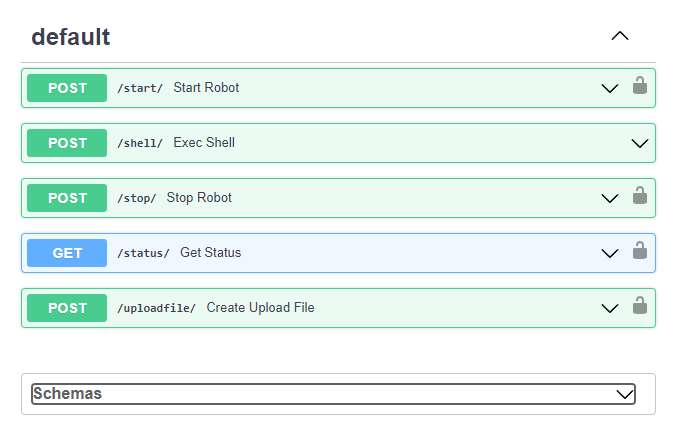
\includegraphics[width=\textwidth]{api-docs.png}
  \caption{API Docs}
  \label{fig:apidocs}
\end{figure}

Bei den implementierten Endpunkten handelt es sich um die in \autoref{fig:apidocs} dargestellten. Folgende Funktionalitäten werden durch die Endpunkte bereitgestellt:

\begin{itemize}
  \item \textbf{/start/}: dieser Endpunkt stellt die Funktionalität bereit, den Roboter unter Verwendung einer vorhandenen Instruktions-Datei zu starten. Dieser Vorgang wird nur dann ausgeführt, wenn noch kein aktiver Fahrvorgang existiert. Ist keine valide Instruktions-Datei vorhanden wird der Vorgang ebenfalls nicht gestartet.
  \item \textbf{/stop/}: dieser Endpunkt stellt die Funktionalität bereit, einen fahrenden Roboter zu stoppen und somit die Ausführung einer Instruktions-Datei zu unterbrechen. Diese Funktion könnte dann von Relevanz sein, wenn das Fahrverhalten Fehler aufweist.
  \item \textbf{/shell/}: dieser Endpunkt liefert die Möglichkeit, reguläre Linux Shell Befehle über die API-Schnittstelle an den verwendeten Raspberry Pi zu übermitteln. Dies ist sowohl mit einzelnen, als auch Aneinanderreihung von Befehlen und Parametern möglich. Hiermit kann der Raspberry beispielsweise neu gestartet oder heruntergefahren werden. Einen Vorteil bietet der Endpunkt insofern, als keine gesonderte SSH-Verbindung für das Ausführen kleinerer Befehle aufgebaut werden muss.
  \item \textbf{/status/}: dieser Endpunkt stellt eine Funktionalität bereit, mit der der aktuelle Status eines Roboters angefragt werden kann. Zum Zeitpunkt der Implementierung beschränkt sich dieser lediglich auf die beiden Zustände \textit{active} und \textit{inactive}. Weiterhin denkbar wären jedoch die Bereitstellung zusätzlicher Informationen wie dem Fortschritt einer aktuell abzuarbeitenden Instruktions-Datei.
  \item \textbf{/uploadfile/}: dieser Endpunkt stellt die Funktionalität bereit, mit der ein Anwender die Instruktionen, der durch den Schwarmintelligenz-Algorithmus errechneten Pfadinformationen, übertragen kann. Es ist zu beachten, dass ein Roboter jeweils einen Datensatz an Instruktionen verarbeiten kann und zum aktuellen Zeitpunkt keine Warteschlange für die Aneinanderreihung mehrerer Instruktions-Dateien vorgesehen ist. Wählt der Anwender eine valide Datei für die Übertragung aus, wird diese nach vorheriger Überprüfung in ein  \textit{/tmp/} Verzeichnis übertragen. Möglicherweise bereits existierende Instruktionen werden hierbei überschrieben. Befindet sich der Roboter zum Zeitpunkt der Anfrage im Zustand \textit{active}, ist ein Übermitteln einer neuen Instruktions-Datei nicht möglich. 
\end{itemize}

\subsection{API Sicherheitsaspekte}
Da der durch den Raspberry bereitgestellte Endpunkt eine Möglichkeit bietet, den Raspberry und die daran angeschlossene Hardware zu steuern, gilt es einige Grundsätze zu beachten, dass durch die Implementierung dieser Schnittstelle keine Schwachstellen offengelegt werden. Besonders, da eine Shell-Kommunikation, zur erweiterten Steuerung, sowie dem Sammeln von Debugging-Informationen genutzt werden soll.

\subsubsection*{API Key Authentifizierung}
Eine gängige Maßnahme um API-Endpunkte gegen unberechtigte Nutzung und gegebenenfalls schadhafte Anfragen zu schützen, ist die Implementierung der Abfrage eines API-Keys zur Authentifizierung des Anwenders \cite{De2017}. Aus diesem Grund werden die Routen durch die Authentifizierung mittels eines API-Keys geschützt, sodass eine Ausführung nur dann erlaubt ist, wenn ein valider API Key im Header der jeweiligen Anfrage mitgeliefert wird. Eine valide Anfrage, wie sie vom Endpunkt des Raspberry Pis akzeptiert wird, ist in \autoref{lst:curl} dargestellt. Die verwendete Länge des API Keys wird anhand der Empfehlungen aus \cite{NISTSP800-57pt3r1} gewählt und in der Implementierung umgesetzt. Weiterhin wird der API Key nicht in den geschriebenen Code, sondern in die Systemumgebungsvariablen des ausführenden Systems integriert. Innerhalb des Codes wird diese Variable zu dem Zeitpunkt aufgerufen, wenn eine Überprüfung des API Keys notwendig ist.

\inputminted{text}{{assets/code/curl.sh}}
\vspace*{-3mm}
\captionof{listing}{\label{lst:curl}Curl API Request}
\vspace*{3mm}

Eine Methode eines API-Endpunkts, der durch die Abfrage des API Keys abgesichert ist, ist in \autoref{lst:sec-api} dargestellt.

\inputminted{python}{{assets/code/run-shell.py}}
\vspace*{-3mm}
\captionof{listing}{\label{lst:sec-api}Geschützter Endpunkt}
\vspace*{3mm}

\subsubsection*{Validierung der JSON Instruktionen}
Neben API-Anfragen, die eine direkte Auswirkungen auf angeschlossene Hardware-Elemente haben können, handelt es sich bei dem Endpunkt \textit{uploadfile} um eine Schnittstelle, bei dem der Anwender einen Request ausführen kann, bei dem der Anwender eine JSON-Datei auf den Raspberry Pi übertragen kann. Die Möglichkeit dieses Vorgangs bietet potenziell die Möglichkeit, Dateien und Dateiformate zu übertragen, welche nicht dafür vorgesehen sind oder sogar schadhafte Auswirkungen auf das Zielsystem haben können. Aus diesem Grund wird eine Validierung der JSON-Datei als notwendig betrachtet. Zudem bietet sich hierdurch der Vorteil, dass die Struktur und der Aufbau der JSON-Datei im gleichen Zug überprüft werden kann und so von vornherein keine inkorrekten Dateien, bei deren Ausführung es zu Fehlern kommen könnte, auf den Raspberry Pi übertragen werden können.

\inputminted{python}{{assets/code/json-check.py}}
\vspace*{-3mm}
\captionof{listing}{\label{lst:json-check}API JSON Validierung}
\vspace*{3mm}

\section{Verarbeitung der Instruktionen}
Damit der Roboter übermittelte Instruktionen umsetzen kann und sich der Roboter fortbewegen kann, wird eine Möglichkeit benötigt, um mit den verwendeten Motoren zu kommunizieren. Hierfür wird durch die Lehrstätte eine Hardware-Komponente bereitgestellt, die diese Anbindung vereinfacht. Das dafür verwendete Grove Base Hat, in \autoref{fig:base-hat} dargestellt, bietet die Möglichkeit mittels einem einzigen Stecker die Anschlüsse \textit{GND, VCC, Signal} zu verbinden. Bei den Instruktionen, die für den Raspberry Pi Roboter benötigt werden, handelt es sich um die Funktionen vorwärts Fahren, rückwärts Fahren, rechts, sowie links Drehen. Diese Manöver werden folgendermaßen implementiert: Die verwendeten Motoren können sich sowohl vorwärts als auch rückwärts drehen. Für den Vorgang des vorwärts Fahrens werden beide Motoren gleichzeitig in Richtung vorwärts angesteuert. Das gleiche Vorgehen wird für den Vorgang des rückwärts Fahrens mit rückwärts Drehungen umgesetzt. Für die Vorgänge der Rechts- sowie Linksdrehung wird jeweils nur ein Motor zur Zeit angesteuert. Eine Drehung in einem bestimmten Winkel wird implementiert, indem zuvor durch Experimente bestimmt wird, wie viele MS ein Motor angesteuert werden muss, um den Roboter beispielsweise um 90 Grad zu drehen. Die Möglichkeit anderer Winkel wird mit diesem ermittelten Faktor errechnet. Für die vorwärts und rückwärts Bewegung muss durch eine Instruktion eine Zeit in Sekunden angegeben werden, für die der Roboter sich bewegen soll. Nach Ablauf dieser Zeit werden die Motoren gestoppt und es können weitere Instruktionen ausgeführt werden.

\section{Umbau des Einplatinencomputers}
Um alle Komponenten des Roboters miteinander zu vereinen wurde eine Plattform mithilfe der Konstruktionssoftware \textit{Fusion 360} erstellt. Die Anforderungen an dieses Modell sind wie folgt:
\begin{itemize}
  \item Die Plattform muss die Möglichkeit bieten, den Raspberry Pi aufzunehmen und zu fixieren.
  \item Es muss eine Möglichkeit geben, die Motoren zu fixieren.
  \item Die Plattform muss die Möglichkeit bieten, die Anschlusskabel der Motoren und des Raspberry Pi zu verbinden.
  \item Der SD-Kartenslot sowie die USB-Anschlüsse des Raspberry Pi müssen zugänglich sein.
\end{itemize}

\begin{figure}[H]
  \centering
  \begin{subfigure}[b]{0.45\textwidth}
    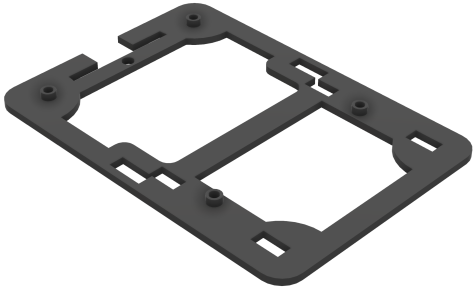
\includegraphics[width=\textwidth]{con-plattform.png}
    \caption{Plattform}
  \end{subfigure}
  \hspace{1cm}
  \begin{subfigure}[b]{0.45\textwidth}
    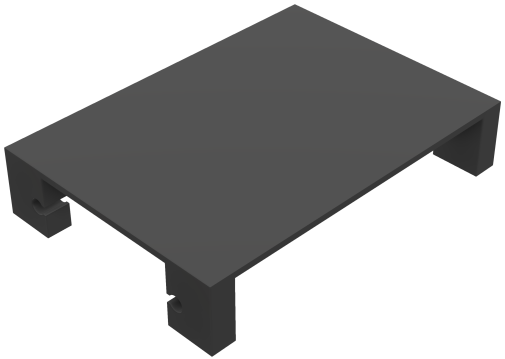
\includegraphics[width=\textwidth]{con-motor-halterung.png}
    \caption{Motor Halterung}
  \end{subfigure}
  \vskip\baselineskip
  \begin{subfigure}[b]{0.45\textwidth}
      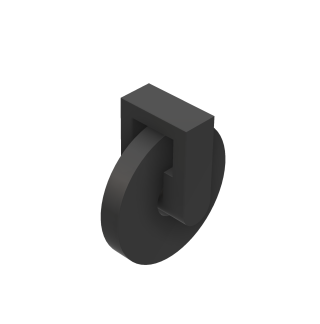
\includegraphics[width=\textwidth]{con-vorderrad.png}
      \caption{Vorderrad}
    \end{subfigure}
    \hspace{1cm}
  \begin{subfigure}[b]{0.45\textwidth}
    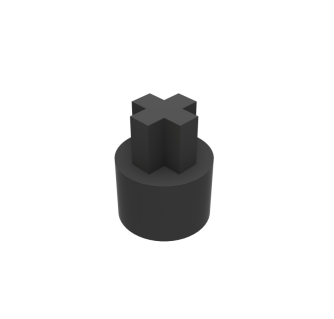
\includegraphics[width=\textwidth]{con-rad-adapter.png}
    \caption{Rad Adapter}
  \end{subfigure}
  \caption{Konstruierte Bauteile \label{fig:konstruktion}}
\end{figure}

Weiterhin müssen an die beiden Motoren die verwendeten Räder angebracht werden. Hierfür wurde ebenfalls ein Adapter konstruiert. Neben den genannten Bauteilen wurde weiterhin ein einzelnes Vorderrad für den Roboter konstruiert. Die Konstruktion der Bauteile ist in \autoref{fig:konstruktion} dargestellt. Nach Fertigstellung sowie mehreren Anpassungen der Konstruktionen wurden die Bauteile mit einem 3D-Drucker hergestellt. Die einzelnen Komponenten wurden miteinander verklebt und anschließend die übrigen Hardware-Komponenten mit Feingewinde-Schrauben befestigt. Der fertige Roboter ist in \autoref{fig:fertiger-roboter} dargestellt. Eine größere Darstellung des Roboters ist zudem dem Anhang in \autoref{sec:darstellungen} zu entnehmen.

\begin{figure}[H]
  \centering
  \begin{subfigure}[b]{0.45\textwidth}
    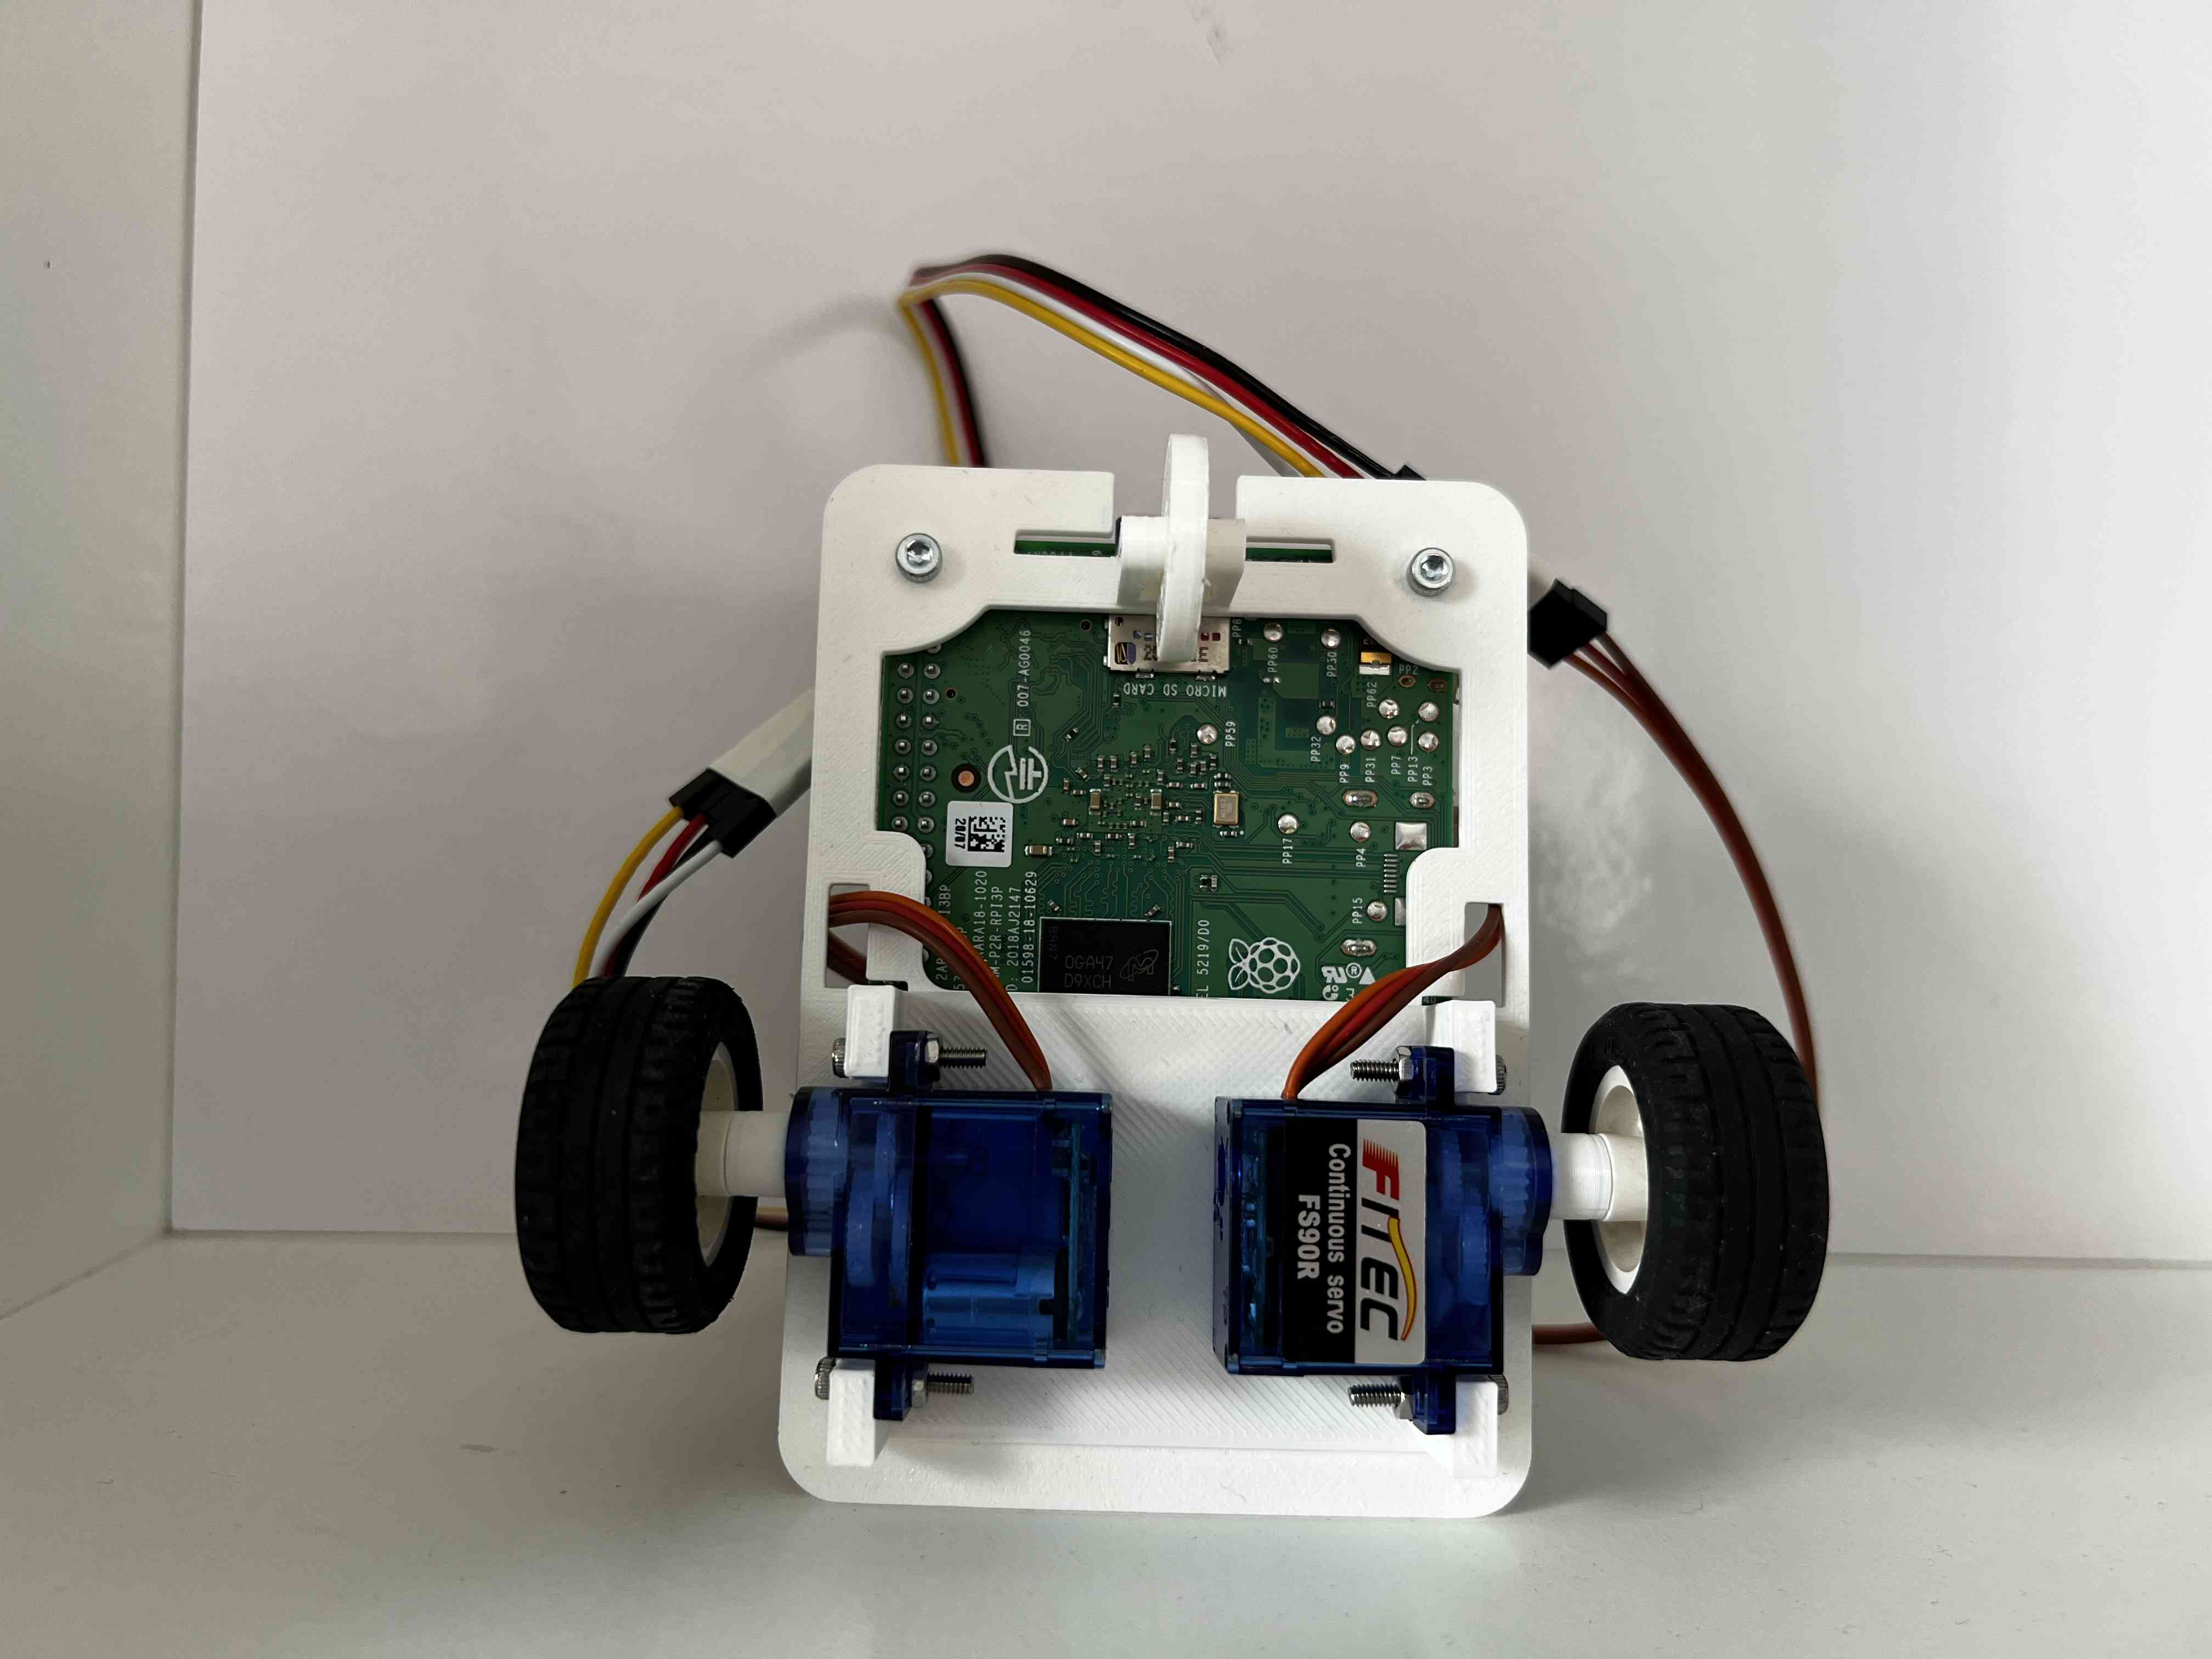
\includegraphics[width=\textwidth]{robot1.jpg}
    \caption{Ansicht von unten}
  \end{subfigure}
  \hspace{1cm}
  \begin{subfigure}[b]{0.45\textwidth}
    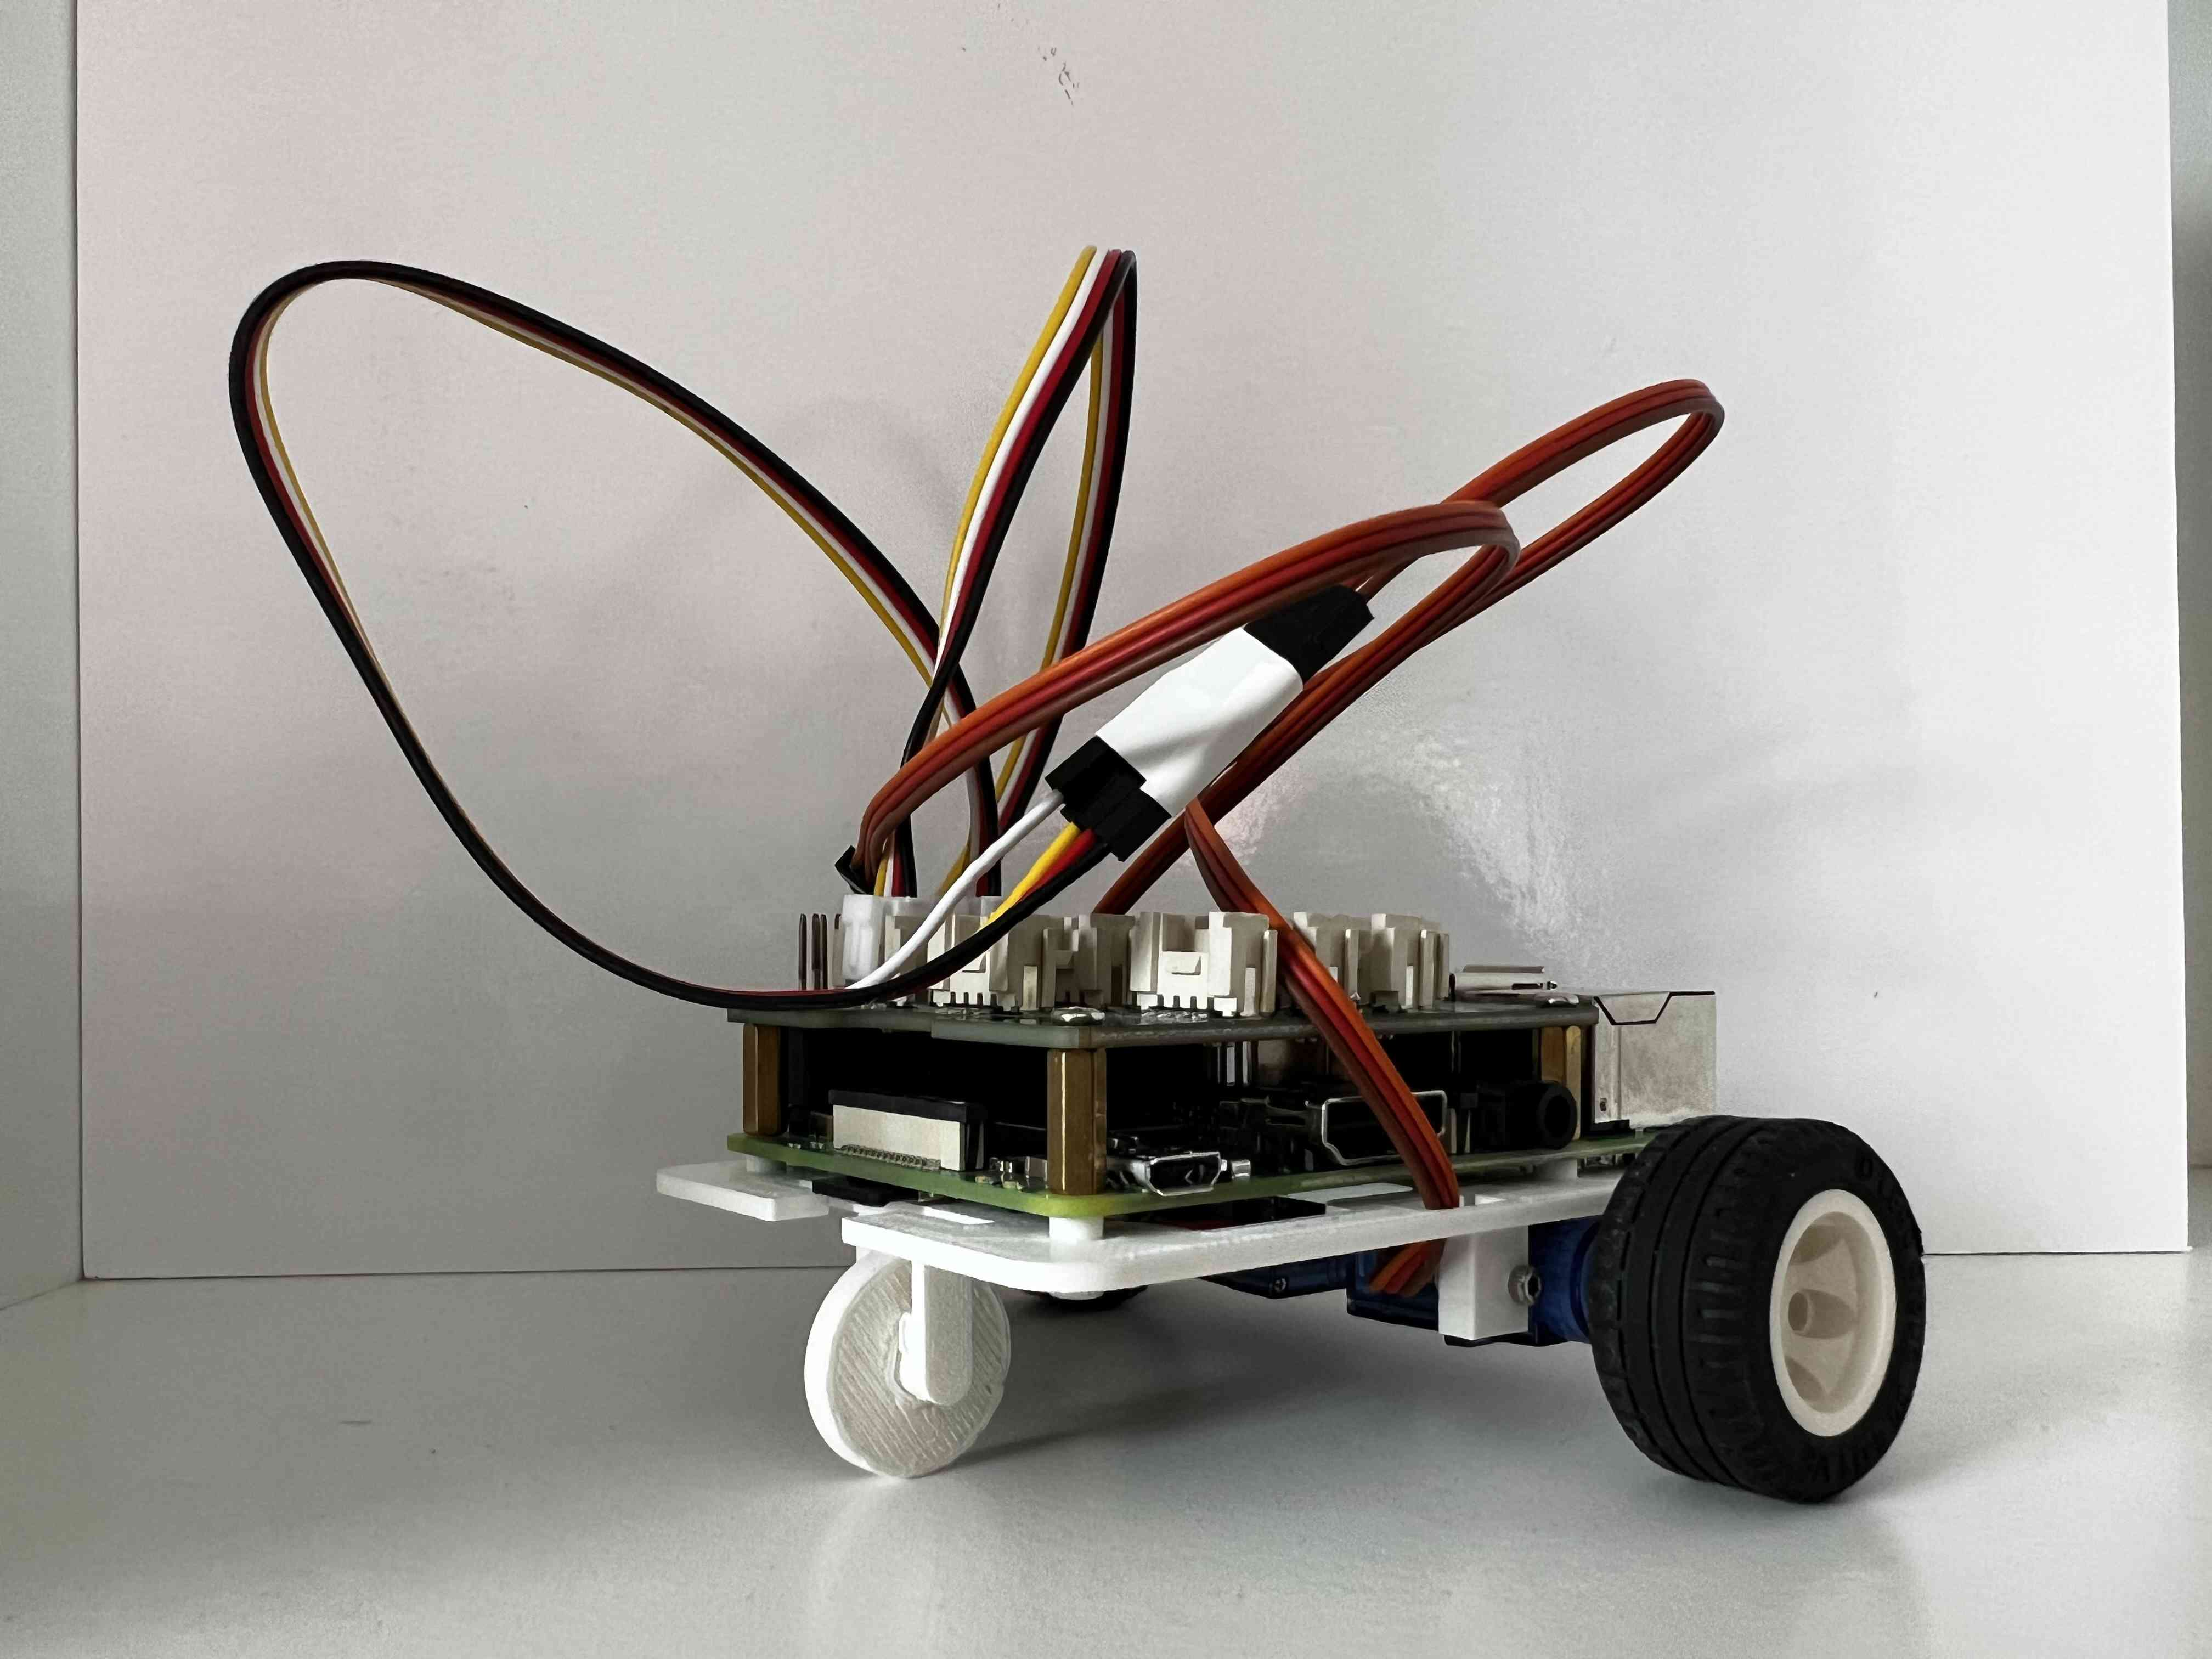
\includegraphics[width=\textwidth]{robot2.jpg}
    \caption{Seitenansicht}
  \end{subfigure}
  \caption{Zusammengebauter Roboter \label{fig:fertiger-roboter}}
\end{figure}

\section{Funktionsweise im Überblick}
Im Folgenden soll eine gesamtheitliche Übersicht geschaffen werden, anhand der die Funktionsweise und Abläufe des Roboters deutlich werden. Die Grundvoraussetzung für die Kommunikation mit dem Roboter ist, dass sich das Gerät, auf dem der Schwarmintelligenz-Algorithmus einen Pfad berechnet und daraus die Instruktionen für den Roboter erstellt, im gleichen Netzwerk angesiedelt sind. Die Kommunikation zwischen den Geräten erfolgt über das Protokoll \textit{HTTP}. Zu Beginn muss an den in \autoref{fig:apidocs} dargestellten Endpunkt \textit{/uploadfile/} eine \textit{JSON}-Datei mit den Instruktionen für den Roboter gesendet werden. Der Aufbau muss wie in \autoref{lst:instructions-json} dargestellt vorliegen. Wenn diese Datei erfolgreich an den Endpunkt des Raspberry Pi übertragen wurde, kann der Roboter gestartet werden. Dies erfolgt über den Endpunkt \textit{/start/}, der im Anschluss der Übertragung aufgerufen werden muss. Nach Aufruf dieses Endpunkts wird auf dem Roboter die zuvor übertragene \textit{JSON}-Datei geladen und anschließend die vorhandenen Instruktionen der Reihenfolge nach durch eine Übersetzungsfunktion ausgeführt. Der vollständige Code zur Ausführung der Instruktionen ist in \autoref{lst:driving_logic} dargestellt. Jeder der Endpunkte gibt eine Rückmeldung, ob die jeweilige Aktion erfolgreich war. 

\inputminted{json}{{assets/code/instructions.json}}
\vspace*{-3mm}
\label{lst:instructions-json}
\captionof{listing}{JSON Instructions}
\vspace*{3mm}

Soll ein neuer Fahrvorgang gestartet werden, muss der Anwender eine neue Datei mit Instruktionen an den Endpunkt senden. Dieser Vorgang ersetzt die zuvor eventuell bereits vorhandene Datei und ermöglicht einen neuen Durchlauf. Der Roboter kann jederzeit über den Endpunkt \textit{/stop/} gestoppt werden.

\section{Probleme bei der Umsetzung}
Im Folgenden sollen Probleme aufgezeigt werden, die bei der Umsetzung, sowohl bei der Konzeption als auch bei der Implementierung, aufgetreten sind. Diese Probleme wurden in der Praxis gelöst und sollen nun in diesem Kapitel erläutert werden.
Damit eine mobile Anwendung des Roboters möglich ist, ist eine Spannungsversorgung mittels eines Akkus notwendig. Der Raspberry Pi 3B+ benötigt eine Versorgungsspannung von 5V, die  über den Micro-USB-Anschluss bereitgestellt werden kann \cite{raspberrypi-docs}. Optimalerweise wird für den Betrieb der Motoren weiterhin eine weitere externe Spanungsquelle verwendet. Diese steht im Rahmen der studentischen Arbeit jedoch nicht zur Verfügung und konnte nicht durch das Inventar der Lehrstätte zur Verfügung gestellt werden. Daher wurde der Rasperry Pi ausschließlich über den Micro-USB-Anschluss mit Strom versorgt, was die Mobilität aufgrund des angeschlossenen Kabels stark einschränkt. 
Bei den vorerst verwendeten Motoren handelt es sich um Motoren, die für den Einsatz in Modellbauanwendungen konzipiert wurden. Hierbei stellte sich zu einem späteren Zeitpunkt der Nachteil heraus, dass diese Motoren nur einen Drehradius von 180° besitzen. Dieser ist für die Bewegung des Roboters nicht ausreichend. Daher wurde ein neuer Motor mit einem Drehradius von 360° verwendet, mit dem die Bewegung des Roboters nun möglich ist.
Weiterhin stellten sich bei der Ansteuerung der Motoren zusätzliche Probleme heraus. Die Ansteuerung der an die GPIO-Pins des Rapsberry angeschlossenen Motoren erfolgt über die Anpassung der \textit{PWM}-Frequenz. Die PWM-Frequenz wird hierbei über die Bibliothek \textit{pigpio} eingestellt. Jedoch stellte sich heraus, dass die Anpassung der PWM-Frequenz nicht zuverlässig funktioniert. Durch die Anpassung sollte es normalerweise möglich sein, die Geschwindigkeit der Motoren zu steuern. Mit der Anpassung war es jedoch lediglich möglich, die Richtung der Drehung der Motoren anzupassen, weswegen eine Anpassung der Fahrgeschwindigkeit des Roboters nicht möglich war. Dies hatte weiterhin zur Folge, dass eine Rechts- sowie Linksdrehung des Roboters nicht während dem Fahren erfolgen kann. Deshalb werden Instruktionen zur Navigation des Rechts- und Linksfahrens nur während des Stillstands des Roboters ausgeführt und Anweisungen hierfür werden inkrementell verarbeitet.